\chapter{Diseño y aspectos de implementación}
\label{cap:diseno}

Este capítulo corresponde a la etapa \textit{Do} del ciclo PDCA y a los objetivos específicos 2 y 3. Describe la arquitectura del núcleo, los contratos de plugin, la capa de abstracción de hardware, los módulos integrados, el rediseño de la interfaz y las iteraciones en que se construyó el sistema.

\section{Arquitectura general}

La nueva versión de EDDIE se organiza en cuatro capas (Figura~\ref{fig:arquitectura}). La \textbf{capa de contratos} (\texttt{contracts/}) define las interfaces abstractas que todo plugin debe implementar. El \textbf{núcleo} (\texttt{orchestrator/}) contiene el orquestador, el cargador de plugins, la fábrica de dispositivos y la traza de ejecución, y no depende de ningún módulo concreto. La \textbf{capa de plugins} (\texttt{hardware/} y \texttt{plugins/}) contiene las implementaciones: sensores reales y simulados, reconocimiento de texto, gestos, rastreo ocular, consistencia, búsqueda y voz. La \textbf{capa de presentación} (\texttt{app/} y \texttt{ui/}) contiene la interfaz de configuración, la pantalla proyectada y el puente \texttt{EddieRuntime} que las conecta con el orquestador.

\begin{figure}[H]
\centering
\begin{tikzpicture}[
  layer/.style={draw=eddietinta, rounded corners=3pt, fill=#1, minimum width=13.4cm, minimum height=1.5cm},
  mod/.style={draw=eddietinta!70, rounded corners=2pt, fill=white, font=\scriptsize, align=center, minimum height=0.75cm, text width=2.3cm},
  lbl/.style={font=\footnotesize\bfseries, anchor=west, text=eddietinta},
  arr/.style={-{Stealth[length=2mm]}, thick, eddieacento}]
\node[layer=eddieacento!8] (ui) at (0,4.7) {};
\node[lbl] at (ui.north west) [below right=1pt] {Presentación (PySide6)};
\node[mod] at (-4.2,4.45) {Menú de\\ configuración};
\node[mod] at (-1.6,4.45) {Pantalla\\ proyectada};
\node[mod] at (1.0,4.45) {EddieRuntime\\ (QTimer, hilos)};
\node[mod] at (3.6,4.45) {Ajustes\\ \texttt{user\_settings}};

\node[layer=eddietinta!6] (core) at (0,2.7) {};
\node[lbl] at (core.north west) [below right=1pt] {Núcleo};
\node[mod] at (-4.2,2.45) {OrchestratorCore};
\node[mod] at (-1.6,2.45) {PluginLoader\\ (\texttt{importlib})};
\node[mod] at (1.0,2.45) {DeviceFactory\\ (real / sim)};
\node[mod] at (3.6,2.45) {ExecutionTrace\\ (JSONL)};

\node[layer=eddietinta!3] (con) at (0,0.9) {};
\node[lbl] at (con.north west) [below right=1pt] {Contratos};
\node[mod, text width=12.6cm, font=\scriptsize] at (0,0.62) {\texttt{PluginBase} --- ICameraSensor $\cdot$ IImageProcessor $\cdot$ IGesturePlugin $\cdot$ IEyeTracker\\ IConsistencyProvider $\cdot$ IWebSearchProvider $\cdot$ ISpeechProvider};

\node[layer=eddieacento!4, minimum height=1.9cm] (pl) at (0,-1.15) {};
\node[lbl] at (pl.north west) [below right=1pt] {Plugins};
\node[mod, text width=1.35cm, font=\tiny] at (-5.3,-1.45) {Cámaras\\ real/sim};
\node[mod, text width=1.35cm, font=\tiny] at (-3.55,-1.45) {OCR};
\node[mod, text width=1.35cm, font=\tiny] at (-1.8,-1.45) {Gestos\\ (3)};
\node[mod, text width=1.35cm, font=\tiny] at (-0.05,-1.45) {Eye tracker\\ (4) + sesión};
\node[mod, text width=1.35cm, font=\tiny] at (1.7,-1.45) {Consistencia\\ (PDF)};
\node[mod, text width=1.35cm, font=\tiny] at (3.45,-1.45) {Búsqueda\\ (LLM)};
\node[mod, text width=1.35cm, font=\tiny] at (5.2,-1.45) {Voz};

\draw[arr] (ui.south) -- (core.north);
\draw[arr] (core.south) -- (con.north);
\draw[arr] (pl.north) -- (con.south);
\node[font=\scriptsize, text=eddieacento, anchor=west] at (0.1,1.75) {usa};
\node[font=\scriptsize, text=eddieacento, anchor=west] at (0.1,-0.03) {implementan};
\end{tikzpicture}
\caption{Arquitectura en capas de EDDIE en Python.}
\label{fig:arquitectura}
\fuente{Elaboración propia.}
\end{figure}

La dependencia va siempre hacia los contratos: el núcleo solo conoce \texttt{PluginBase} y los contratos de dominio, y los plugins solo conocen los contratos que implementan. Esto permite agregar un plugin sin modificar el núcleo (RNF-04) y reemplazar un dispositivo por su versión simulada sin modificar los plugins que lo consumen (RNF-05). A diferencia de EDDIE-2023 (Figura~\ref{fig:arq_legada}), existe un único camino de carga para todos los módulos.

\section{Contratos de plugin}

Todo plugin hereda de \texttt{PluginBase}, que define tres métodos obligatorios, \texttt{initialize(config)}, \texttt{execute()} y \texttt{release()}, y la propiedad \texttt{name}. Sobre esa base, cada dominio tiene un contrato con las operaciones que el resto del sistema necesita (Tabla~\ref{tab:contratos}). Dos interfaces auxiliares resuelven el flujo de datos entre plugins: \texttt{ICameraFrameConsumer}, para los plugins que reciben un sensor de cámara inyectado, e \texttt{ICycleResultConsumer}, para los que necesitan los resultados de los demás plugins del mismo ciclo.

\begin{table}[H]
\centering
\caption{Contratos de plugin y sus implementaciones.}
\label{tab:contratos}
\footnotesize
\begin{tabularx}{\textwidth}{>{\raggedright\arraybackslash}p{3.7cm} >{\raggedright\arraybackslash}X >{\raggedright\arraybackslash}p{4.0cm}}
\toprule
\textbf{Contrato} & \textbf{Operaciones principales} & \textbf{Implementaciones} \\ \midrule
\texttt{PluginBase} & \texttt{initialize}, \texttt{execute}, \texttt{release}, \texttt{name} & Todos los plugins \\ \midrule
\texttt{ICameraSensor} & \texttt{capture\_frame}, \texttt{get\_latest\_frame} & \texttt{CameraSensorPlugin}, \texttt{MockCameraSensor} \\ \midrule
\texttt{IImageProcessor} & \texttt{preprocess}, \texttt{extract\_text}, \texttt{recognize\_highlighted\_text}, \texttt{get\_precision\_recall} & \texttt{ImageProcessorPlugin} \\ \midrule
\texttt{IGesturePlugin} & \texttt{detect\_gesture}, \texttt{set\_calibration}, \texttt{mark\_selection\_start/end}, \texttt{capture\_selection} & \texttt{ColorPenPlugin}, \texttt{HandSkinPlugin}, \texttt{MousePlugin} \\ \midrule
\texttt{IEyeTracker} & \texttt{get\_gaze\_point}, \texttt{is\_connected}, \texttt{get\_latency\_ms} & \texttt{EyeTrackerPlugin} (GazePoint, TheEyeTribe, GazeCloud), \texttt{EyeTrackerMock} \\ \midrule
\texttt{IConsistencyProvider} & \texttt{load\_document}, \texttt{add\_highlight}, \texttt{get\_annotations}, \texttt{search\_text}, marcadores y comentarios & \texttt{ConsistencyPlugin} \\ \midrule
\texttt{IWebSearchProvider} & \texttt{search\_encyclopedia}, \texttt{search\_definition}, \texttt{translate\_text}, \texttt{search\_image}, \texttt{search\_video} & \texttt{LLMSearchPlugin} (Gemini) \\ \midrule
\texttt{ISpeechProvider} & \texttt{speak}, \texttt{stop\_speaking}, \texttt{start\_listening}, \texttt{stop\_listening} & \texttt{SpeechPlugin} \\ \bottomrule
\end{tabularx}
\fuente{Elaboración propia a partir de \texttt{contracts/}.}
\end{table}

\section{Núcleo orquestador}

\subsection{Ciclo de vida}

El \texttt{OrchestratorCore} lee \texttt{config/plugins.json}, superpone los ajustes del usuario, carga los plugins con el \texttt{PluginLoader} y los inicializa respetando sus dependencias (por ejemplo, el reconocimiento de texto depende de la cámara de texto). En cada ciclo llama a \texttt{execute()} de cada plugin, primero los productores y luego los consumidores de resultados, y mide la latencia de cada uno. Al cerrar, libera los plugins en orden inverso al de inicialización. El Algoritmo~\ref{alg:ciclo} resume el ciclo; el aislamiento de fallos está en las líneas marcadas con \texttt{try}.

\begin{algorithm}[H]
\caption{Ciclo de vida del orquestador.}
\label{alg:ciclo}
\SetKwInOut{Input}{Entrada}\SetKwInOut{Output}{Salida}
\Input{archivo \texttt{plugins.json}, ajustes del usuario}
\Output{resultados por ciclo, métricas de latencia, traza}
$C \leftarrow$ leer configuración y superponer ajustes\;
\ForEach{entrada $e \in C$ habilitada}{
  $clase \leftarrow$ \texttt{DeviceFactory.resolve}$(e)$ \tcp*{real o simulada}
  \textbf{try} cargar $clase$ con \texttt{importlib} \textbf{except} registrar \texttt{load\_failed}\;
}
\ForEach{plugin $p$ cargado, en orden de dependencias}{
  inyectar sensor declarado si $p$ es \texttt{ICameraFrameConsumer}\;
  \textbf{try} $p.\texttt{initialize}(config_p)$ \textbf{except} registrar falla y continuar\;
}
\While{el sistema esté activo}{
  $R \leftarrow \emptyset$\;
  \ForEach{plugin activo $p$ (productores primero, consumidores al final)}{
    $t_0 \leftarrow$ \texttt{perf\_counter}()\;
    \lIf{$p$ es \texttt{ICycleResultConsumer}}{$p.\texttt{consume\_cycle\_results}(R)$}
    \textbf{try} $R[p] \leftarrow p.\texttt{execute}()$ \textbf{except} $R[p] \leftarrow$ error, registrar\;
    registrar latencia $t-t_0$; advertir si supera 8,3~ms\;
  }
}
\ForEach{plugin $p$ en orden inverso}{\textbf{try} $p.\texttt{release}()$ \textbf{except} registrar\;}
\end{algorithm}

Además del ciclo, el orquestador ofrece tres operaciones que necesita la interfaz: \texttt{invoke(plugin, método, …)}, que ejecuta una operación bajo demanda (por ejemplo, reconocer el texto resaltado o buscar una definición) con el mismo aislamiento de fallos y midiendo su latencia; \texttt{restart\_plugin}, que reinicia un plugin con una configuración nueva y reconecta a sus consumidores; y \texttt{stop\_plugin}. Cada acción queda registrada en una traza JSONL que sirve de evidencia para la evaluación.

\subsection{Configuración declarativa}

Todos los plugins se declaran en un único archivo. Cada entrada indica la clase, la implementación simulada si es un dispositivo, las dependencias y la configuración:

\begin{verbatim}
{ "name": "ImageProcessor",
  "class": "plugins.image_processor_plugin.ImageProcessorPlugin",
  "enabled": true,
  "dependencies": {"camera_sensor": "TextCamera"},
  "config": {"ocr_language": "spa+eng", "rotate_180": true} }
\end{verbatim}

Agregar un módulo consiste en escribir la clase y agregar una entrada; si la clase no existe o tiene un error, el plugin queda registrado como fallido y el resto del sistema arranca igual, que es exactamente el caso que en EDDIE-2023 detenía la aplicación (E50). Los ajustes del usuario (cámara elegida, PDF, eye tracker) se guardan en un archivo aparte, \texttt{config/user\_settings.json}, con las mismas claves que usaba \texttt{Settings2} en C\#, y se superponen al cargar sin modificar \texttt{plugins.json}.

\subsection{Capa de abstracción de hardware}

La \texttt{DeviceFactory} decide, para cada dispositivo que declara \texttt{simulated\_class}, si se carga la implementación real o la simulada. El modo se elige con la variable de entorno \texttt{EDDIE\_DEVICE\_MODE} (\texttt{real} o \texttt{sim}) o por dispositivo en su configuración. Las implementaciones simuladas generan señales con verdad terreno conocida: \texttt{MockCameraSensor} entrega una página con texto resaltado, un lápiz o una mano en posiciones conocidas, y \texttt{EyeTrackerMock} una trayectoria de mirada. Esto permite ejecutar el sistema completo y las pruebas automatizadas sin el laboratorio (RNF-05) y, en una sesión real, distinguir una falla del sensor de una falla del software: si el sistema funciona en modo simulado y no en el real, el problema está en el dispositivo o su conexión.

\subsection{Integración con la interfaz}

\texttt{EddieRuntime} conecta el orquestador con la interfaz. Un temporizador de Qt ejecuta \texttt{execute\_cycle()} a 30~Hz en el hilo de la interfaz, mientras que los sensores capturan en hilos propios, de modo que un ciclo nunca espera a la cámara. Las acciones lentas (OCR, consulta al modelo de lenguaje, guardado del PDF, voz) se ejecutan con \texttt{invoke} en un conjunto de hilos de trabajo y su resultado vuelve a la interfaz por una señal. Este esquema reemplaza los hilos y ventanas de carga \textit{ad hoc} de EDDIE-2023.

\section{Módulos integrados}

\begin{description}
  \item[Reconocimiento de texto.] \texttt{ImageProcessorPlugin} recibe la cámara de texto, localiza la zona resaltada, la recorta y la transcribe con Tesseract (\texttt{spa+eng}). También calcula precisión y recall contra una lista de palabras esperadas, la métrica de la propuesta para la verificación funcional.
  \item[Interacción gestual.] Tres plugins implementan \texttt{IGesturePlugin}: lápiz de color, mano y mouse. Comparten la calibración de cuatro puntos, la selección de un fragmento y su captura, y una opción común para rotar la imagen 180° cuando la cámara está montada invertida (hallazgo H-01).
  \item[Rastreo ocular.] \texttt{EyeTrackerPlugin} implementa los protocolos de GazePoint (Open Gaze API, TCP 4242), TheEyeTribe (TCP 6555) y GazeCloud (WebSocket 3000). \texttt{GazeSessionPlugin} registra la sesión de mirada en CSV con las columnas de EDDIE-2023 y el clic por permanencia.
  \item[Consistencia.] \texttt{ConsistencyPlugin} mantiene el PDF abierto y sincroniza resaltados, comentarios, marcadores y figuras en ambos sentidos con PyMuPDF. Cada guardado escribe una copia completa y reemplaza el original (hallazgo H-02).
  \item[Búsqueda.] \texttt{LLMSearchPlugin} implementa los cinco servicios de \texttt{IWebSearchProvider} con Gemini 2.5 Flash. La clave se lee de \texttt{config/secrets.json} o de la variable \texttt{GEMINI\_API\_KEY}, que no se versionan.
  \item[Voz.] \texttt{SpeechPlugin} lee los resultados con \texttt{pyttsx3} y escucha los comandos con \texttt{SpeechRecognition}.
\end{description}

\section{Diseño de la interfaz}

La interfaz de EDDIE-2023 se reconstruyó primero como réplica de los formularios WinForms (a partir de los archivos \texttt{.Designer.cs}) para no perder ningún control, y luego se rediseñó conservando todos los controles y flujos con el mismo nombre y comportamiento (RNF-06). Los criterios del rediseño provienen de la evaluación de \citet{ibaceta2023evaluacion} y de la operación en la sala:

\begin{itemize}
  \item \textbf{Sin amarillo fuera del resaltado.} La cámara detectaba el botón de resaltado de la proyección en lugar del texto (EFD2). La paleta usa tinta azul oscura (\#1B2440) y un acento verde azulado (\#0B7A87); el amarillo queda reservado para el resaltado, que es lo que el OCR busca.
  \item \textbf{Controles de la proyección en la franja superior.} TheEyeTribe no detectaba la parte inferior de la proyección (E49) y el reconocimiento de texto fallaba lejos de la cámara (EFD4), por lo que los botones que se activan con la mirada se ubican en la franja superior. La zona de lectura y las cruces de calibración conservan su posición original, porque los algoritmos de reconocimiento dependen de ellas.
  \item \textbf{Estado real de cada módulo.} La pantalla de inicio muestra los pasos para preparar la sesión y el estado de cada módulo según el orquestador (U1), y los mensajes son avisos no modales que no detienen la lectura (U3).
  \item \textbf{Calibración desde el sensor.} Los puntos de calibración gestual se copian de la lectura actual del sensor en lugar de escribirse a mano (U2).
  \item \textbf{Español en toda la interfaz} (E14).
\end{itemize}

Las Figuras~\ref{fig:ui_inicio} a~\ref{fig:ui_proyeccion} muestran la interfaz final; la comparación con EDDIE-2023 está en el Apéndice~\ref{ap:interfaz}.

\begin{figure}[H]
\centering
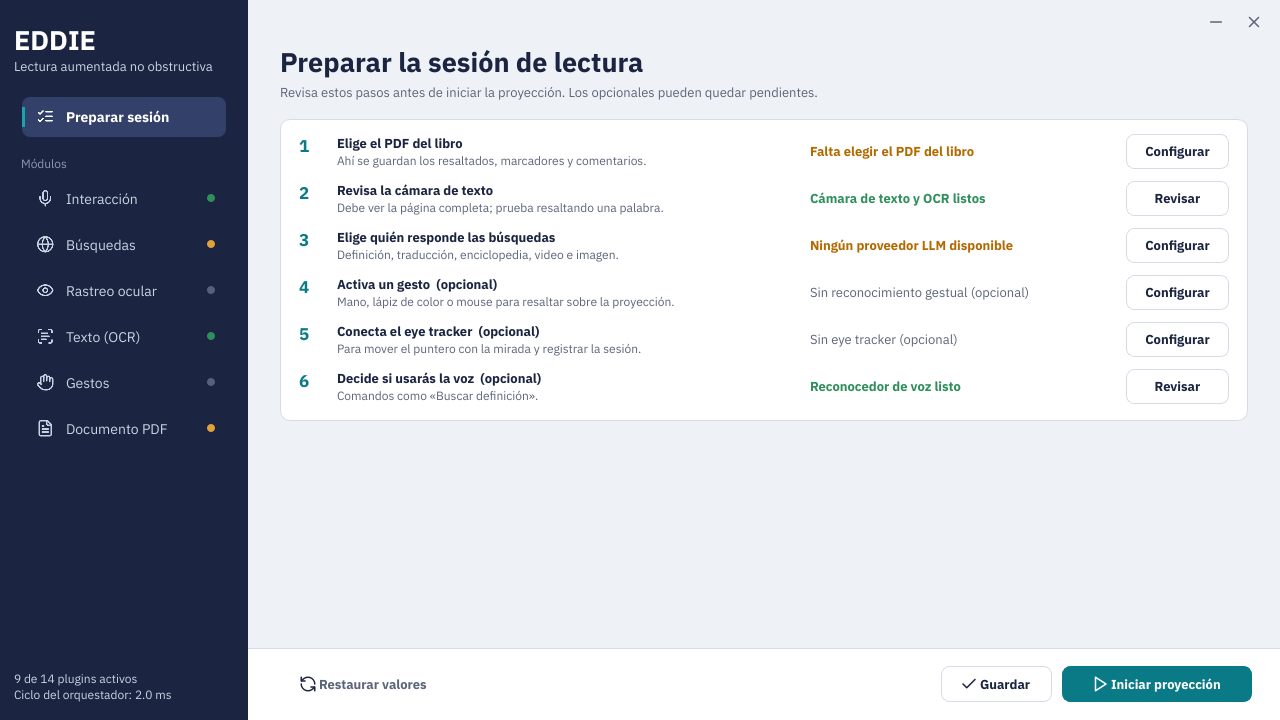
\includegraphics[width=0.85\textwidth]{figuras/00_menu_settings.png}
\caption{Pantalla de inicio con los pasos de preparación y el estado de cada módulo.}
\label{fig:ui_inicio}
\fuente{Elaboración propia (captura del avance P-07 con dispositivos simulados).}
\end{figure}

\begin{figure}[H]
\centering
\begin{minipage}{0.49\textwidth}\centering
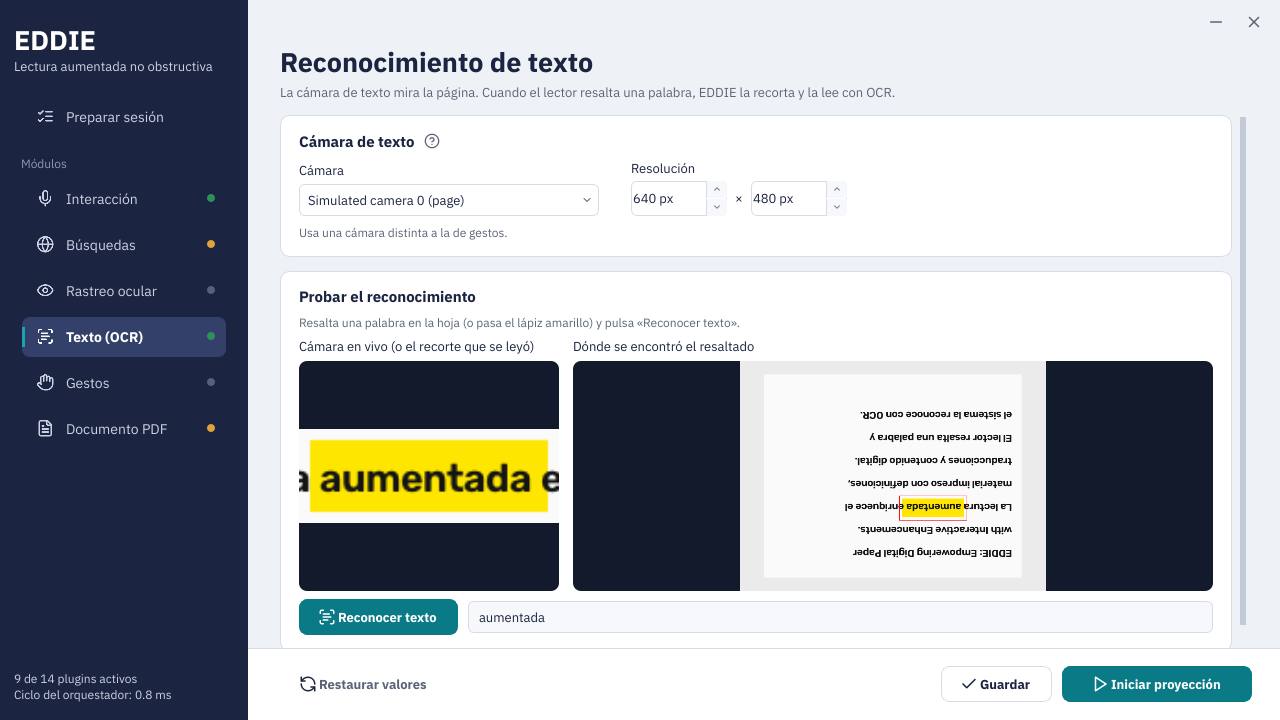
\includegraphics[width=\linewidth]{figuras/01_text.png}
\end{minipage}\hfill
\begin{minipage}{0.49\textwidth}\centering
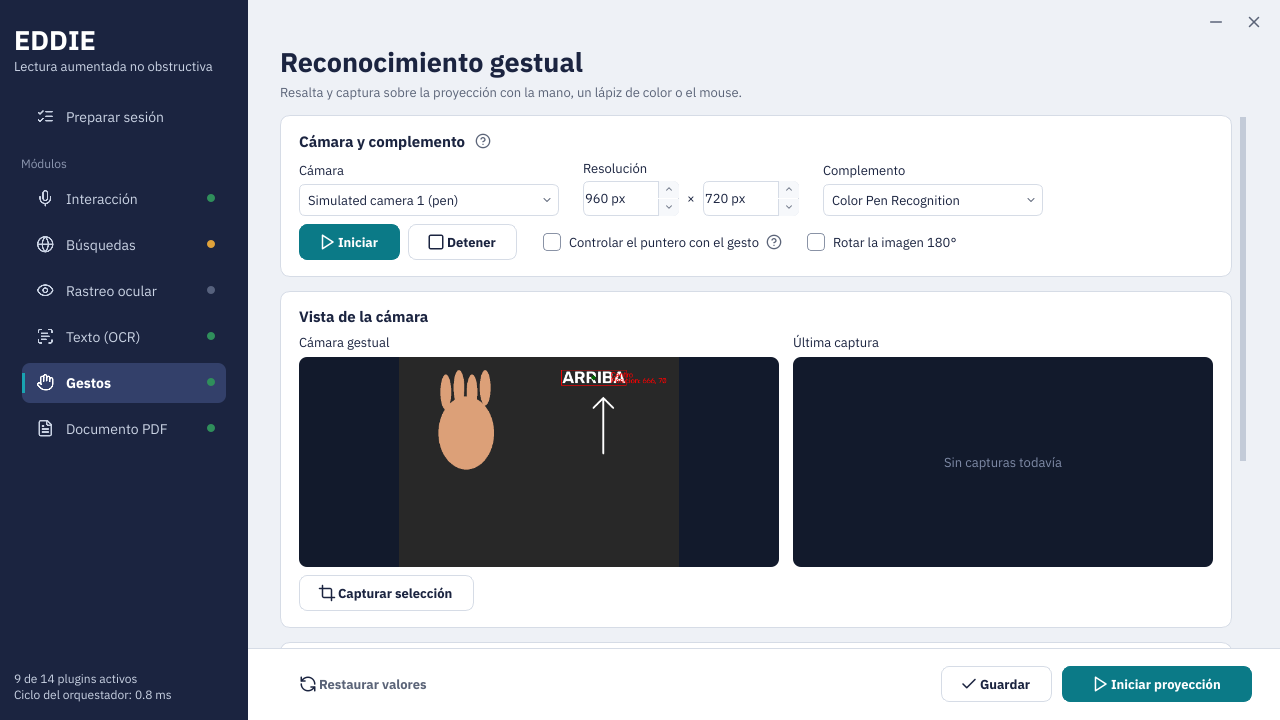
\includegraphics[width=\linewidth]{figuras/03_gesture_lapiz.png}
\end{minipage}
\caption{Configuración del reconocimiento de texto (izquierda) y de la interacción gestual con lápiz (derecha).}
\label{fig:ui_texto_gestos}
\fuente{Elaboración propia (capturas del avance P-07).}
\end{figure}

\begin{figure}[H]
\centering
\begin{minipage}{0.49\textwidth}\centering
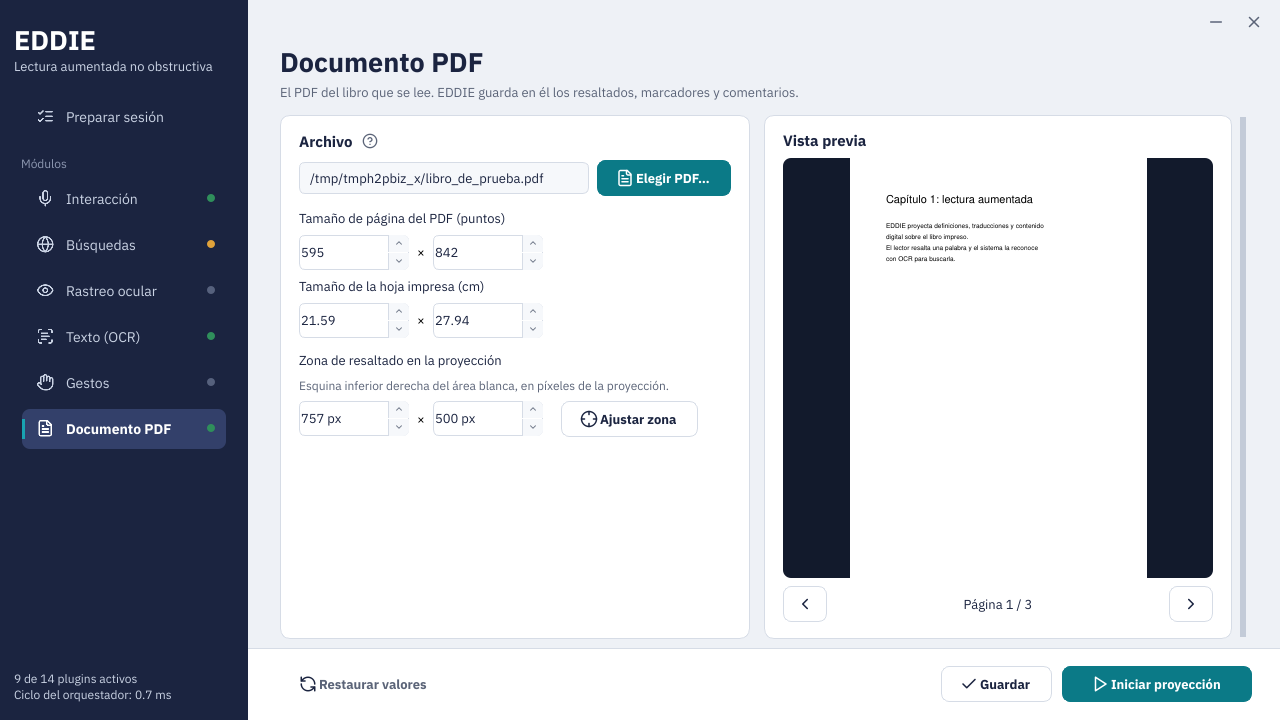
\includegraphics[width=\linewidth]{figuras/02_page.png}
\end{minipage}\hfill
\begin{minipage}{0.49\textwidth}\centering
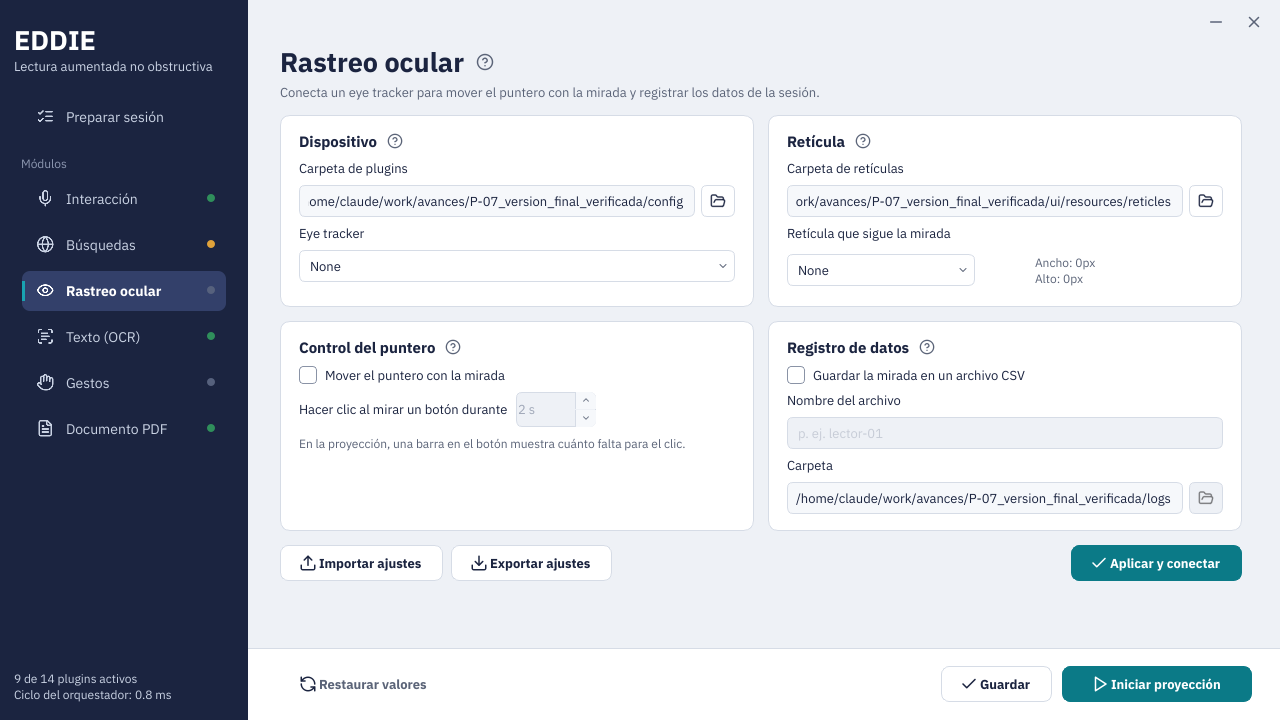
\includegraphics[width=\linewidth]{figuras/04_eye.png}
\end{minipage}
\caption{Configuración del documento PDF (izquierda) y del rastreo ocular (derecha).}
\label{fig:ui_pdf_ojo}
\fuente{Elaboración propia (capturas del avance P-07).}
\end{figure}

\begin{figure}[H]
\centering
\begin{minipage}{0.49\textwidth}\centering
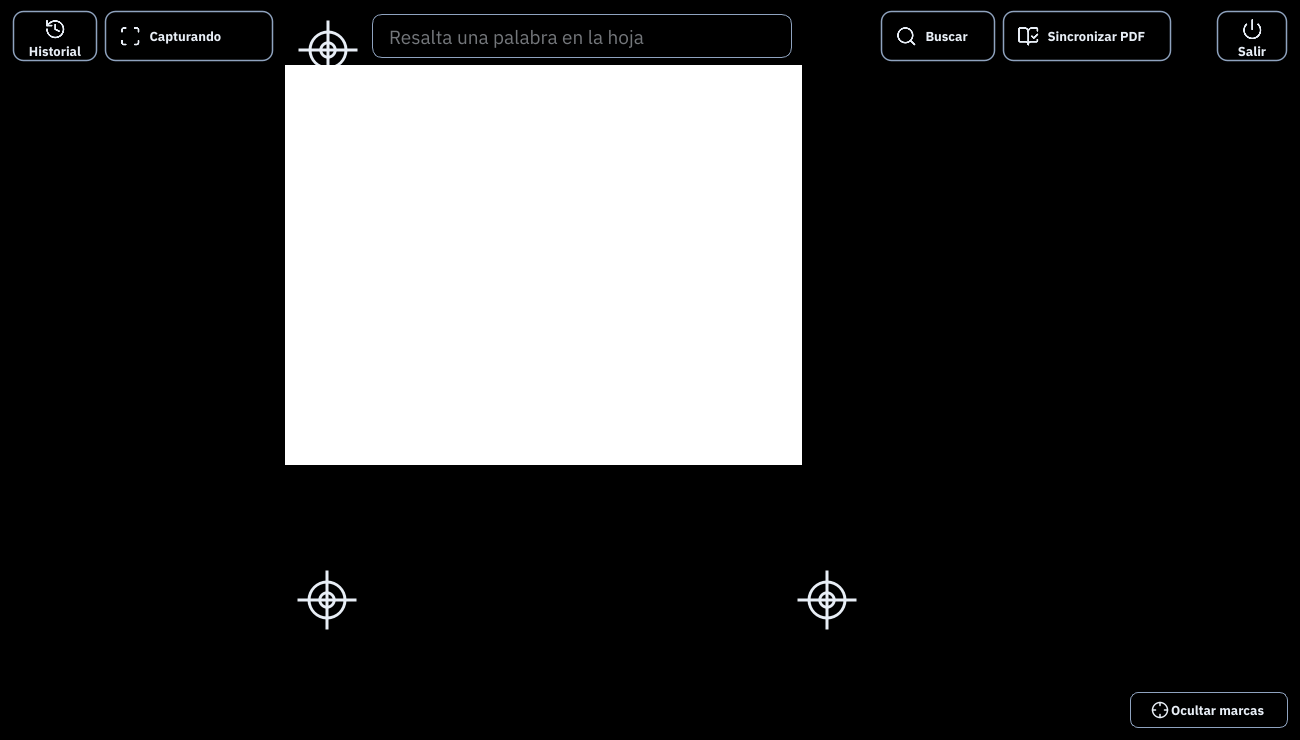
\includegraphics[width=\linewidth]{figuras/10_proyeccion.png}
\end{minipage}\hfill
\begin{minipage}{0.49\textwidth}\centering
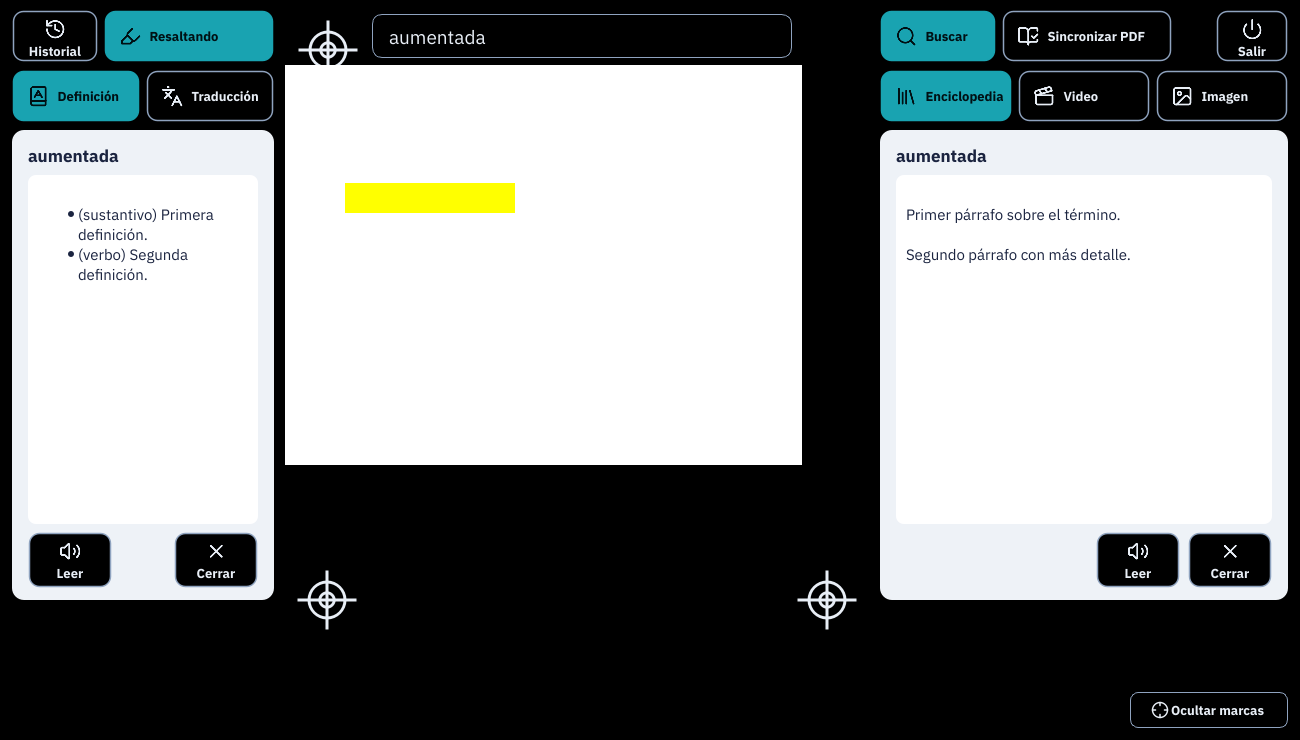
\includegraphics[width=\linewidth]{figuras/11_proyeccion_busqueda.png}
\end{minipage}
\caption{Pantalla proyectada: controles en la franja superior (izquierda) y resultado de una búsqueda (derecha).}
\label{fig:ui_proyeccion}
\fuente{Elaboración propia (capturas del avance P-07 con un modelo de lenguaje de prueba).}
\end{figure}

\section{Iteraciones de desarrollo}

El sistema se construyó en ocho avances, cada uno con su código completo, pruebas y evidencias reproducibles (Tabla~\ref{tab:avances}). P-00 corresponde a los prototipos desechables del Capítulo~\ref{cap:analisis}; P-01 a P-06 integran el núcleo y los módulos en el orden de menor a mayor dependencia del hardware; P-07 es la versión verificada. La interfaz se incorpora desde P-03 y muestra, en cada avance, solo los módulos ya integrados: los demás aparecen deshabilitados con la etiqueta del avance en que se integran. Las fichas de cada avance, con sus objetivos y requisitos, están en el Apéndice~\ref{ap:avances}.

\begin{table}[H]
\centering
\caption{Avances del desarrollo y resultados de sus pruebas.}
\label{tab:avances}
\footnotesize
\begin{tabularx}{\textwidth}{l >{\raggedright\arraybackslash}X c c c c}
\toprule
\textbf{Avance} & \textbf{Contenido} & \textbf{PDCA} & \textbf{Pruebas} & \textbf{Fallos esperados} & \textbf{Cobertura} \\ \midrule
P-00 & Prototipos desechables y mediciones & Plan & --- & --- & --- \\
P-01 & Núcleo orquestador y contratos & Do & \PUnoPruebas & \PUnoXfail & \PUnoCobertura\% \\
P-02 & Capa de hardware y consistencia & Do & \PDosPruebas & \PDosXfail & \PDosCobertura\% \\
P-03 & Reconocimiento de texto e interfaz & Do & \PTresPruebas & \PTresXfail & \PTresCobertura\% \\
P-04 & Interacción gestual & Do & \PCuatroPruebas & \PCuatroXfail & \PCuatroCobertura\% \\
P-05 & Rastreo ocular & Do & \PCincoPruebas & \PCincoXfail & \PCincoCobertura\% \\
P-06 & Proyección, búsqueda con LLM y voz & Do & \PSeisPruebas & \PSeisXfail & \PSeisCobertura\% \\
P-07 & Versión final verificada & Check/Act & \PSietePruebas & \PSieteXfail & \PSieteCobertura\% \\ \bottomrule
\end{tabularx}
\fuente{Elaboración propia a partir de \texttt{evidencias/} de cada avance.}
\end{table}

Los fallos esperados (\textit{xfail}) son pruebas que documentan un defecto conocido: en los avances en que el defecto existe la prueba se marca como fallo esperado, y en P-07, con la corrección aplicada, pasa a aprobada. Así cada corrección queda respaldada por una prueba que demuestra el problema y su solución (Sección~\ref{sec:hallazgos}).
